\section{Simulations}

In order to study the long-term behavior of the noise-perturbed sim-max games, we conducted computer simulations for different combinations of initial parameters.
Namely, we were interested in investigating the impact of different values of impairment and its relation with the size of the state space.
\mytodo{JPC}{Justify why size of state space is interesting}

\subsection{Metrics}
\label{sec:metrics}
To be able to quantitively analyze the results of our simulations, we define a number of metrics to capture different characteristics of sim-max languages.

\paragraph{Entropy.}
This classic information-theoretic metric captures the amount of uncertainty in a signaling strategy.
The most natural way to define it is in terms of mixed strategies rather than behavioral strategies.
Let us recall that mixed sender (receiver) strategies are functions $\Smixed \in \Delta(\Messgs^\States)$ ($\Rmixed \in (\Acts^\Messgs)$).
We can define the entropy of a sender strategy as
\begin{align*}
  E(\Smixed) = \sum_{\Spure \in \Messgs^\States} \Smixed(\Spure) \cdot \log(\Smixed(\Spure))
\end{align*} 
and the entropy of a receiver strategy as
\begin{align*}
  E(\Rmixed) = \sum_{\Rpure \in \Acts^\Messgs} \Rmixed(\Rpure) \cdot \log(\Rmixed(\Rpure)) \,.
\end{align*} 
These metrics are computationally expensive to calculate, since the size of the domain over which the sum is computed grows exponentially with the number of choice points.
Therefore, we converted\footnote{See Appendix~\ref{sec:proofs}.} the above definitions into equivalent metrics defined in terms of behavioral strategies.
These are as follows:
\begin{align*}
  E(\Sstrat) = -\sum_{\state \in \States} \sum_{\messg \in \Messgs} \Sstrat(\messg \probbar \state) \cdot \log(\Sstrat(\messg \probbar \state))
\end{align*} 
\begin{align*}
  E(\Rstrat) = -\sum_{\messg \in \Messgs} \sum_{\act \in \Acts} \Rstrat(\act \probbar \messg) \cdot \log(\Rstrat(\act \probbar \messg)) \,.
\end{align*}
The metrics are lower bounded by $0$ and upper bounded by, respectively, $\log(|\Messgs^\States|) = |\States| \cdot \log(|\Messgs|)$ and $\log(|\Acts^\Messgs|) = |\Messgs| \cdot \log(|\Acts|)$, thus we can normalize them by dividing by these values.

\paragraph{Informativity.}
\mytodo{JPC}{Informativity is perhaps a bad name for the receiver...}
The quantity of information in a signal is an old notion that also goes back to the start of information theory.
Skyrms~\citet[ch.~3]{Skyrms2010:Signals} discusses its use in the context of signaling games.
The main idea is that we can quantify the amount of information about a state $\state$ in a message $\messg$ via the relation between the probability of the state given the message $\Pr(\state \,|\, \messg)$ and the unconditional probability of the state $\Pr(\state)$.
Following Bayes' theorem, we can express $\Pr(\state \,|\, \messg)$ as $\frac{\Pr(\state) \cdot \Pr(\messg \,|\, \state)}{\Pr(\messg)}$.
We then have $\Pr(\messg \,|\, \state) = \Sstrat(\state,\messg)$ and $\Pr(\messg) = \sum_{\state^\prime \in \States} \Pr(\state^\prime) \cdot \Sstrat(\state^\prime,\messg)$.
Finally, we equate sender infomativity with the average overall information about states in each signal.
Based on the definition by Skyrms~\citet[p.~36]{Skyrms2010:Signals}, and the considerations above, we define sender informativity as follows:
\begin{align*}
  I(\Sstrat) = \frac{1}{|\Messgs|} \sum_{\messg \in \Messgs} \sum_{\state \in \States} \frac{\Pr(\state) \cdot \Sstrat(\state,\messg)}{\sum_{\state^\prime \in \States} \Pr(\state^\prime) \cdot \Sstrat(\state^\prime,\messg)} \cdot \log \left(\frac{\Sstrat(\state,\messg)}{\sum_{\state^\prime \in \States} \Pr(\state^\prime) \cdot \Sstrat(\state^\prime,\messg)} \right) \,.
\end{align*}
Conversely, we can quantify the amount of information about an act in a message.
We equate receiver informativity with the average overall information about acts in each signal.
Based on Skyrms' definition~\citet[p.~39]{Skyrms2010:Signals}, we define receiver informativity as follows:
\begin{align*}
  I(\Sstrat,\Rstrat) = \frac{1}{|\Messgs|} \sum_{\messg \in \Messgs} \sum_{\act \in \Acts} \Rstrat(\messg,\act) \cdot \log \left(\frac{\Rstrat(\messg,\act)}{\sum_{\state \in \States} \Pr(\state) \cdot \sum_{\messg^\prime \in \Messgs} \Sstrat(\state,\messg^\prime) \cdot \Rstrat(\messg^\prime,\act)} \right) \,.
\end{align*}
Both metrics are bounded between $0$ and $1$.

\paragraph{Voronoiness.}
This metric aims to quantify how close a strategy is to being a part of a Voronoi tessallation of the state space.
Recalling the results by \cite{Jager2007}, the stable outcomes of a population of agents playing a similarity-maximization game using pure strategies and evolving according to the replicator dynamics are those where ``the sender strategy is consistent with the Voronoi tessallation that is induced by the image of the receiver strategy.''~(\cite{Jager2007}, p. 562).
\mytodo{JPC}{Explain further?}
Given we are working with behavioral strategies, rather than pure strategies, and that we perform numerical simulations, rather than calculate analytical results, instead of looking into a binary criterion of whether a simulation result is such a Voronoi tessallation of the state space or not, we want a more progressive metric to characterize that in terms of degrees.
With that in mind, and given that this metric only makes sense for $\Acts = \States$, we define Voronoiness as follows.
Let $\pi(\Rstrat, \messg) = \argmax_{\state \in \States}\Rstrat(\messg,\state)$ be the prototype of a message $\messg \in \Messgs$, then
\begin{multline*}
  V(\Sstrat, \Rstrat) = \sum_{\state \in \States} \sum_{\messg_1 \in \Messgs} \sum_{\messg_2 \in \Messgs} \textrm{if } s(\state, \pi(\Rstrat, \messg_1)) > s(\state, \pi(\Rstrat, \messg_2)) \bicond \Sstrat(\state, \messg_1) > \Sstrat(\state, \messg_2) \textrm{ then } 1 \textrm{ else } 0
\end{multline*}
is the Voronoiness of the sender strategy $\Sstrat$ given the receiver strategy $\Rstrat$ and
\begin{align*}
  V(\Rstrat) = \sum_{\messg \in \Messgs} \sum_{\state_1 \in \States} \sum_{\state_2 \in \States} \textrm{if } s(\state_1, \pi(\Rstrat, \messg)) > s(\state_2, \pi(\Rstrat, \messg)) \bicond \Rstrat(\messg, \state_1) > \Rstrat(\messg, \state_2) \textrm{ then } 1 \textrm{ else } 0
\end{align*}
is the Voronoiness of the receiver strategy $\Rstrat$.
\mytodo{JPC}{Give some intuitions on these?}
The metrics are lower bounded by $0$ and upper bounded by, respectively, $|\States| \times |\Messgs|^2$ and $|\Messgs| \times |\States|^2$, thus we can normalize them by dividing by these values.

\subsection{Methodology}
\newcommand{\impairment}{\alpha}
In our simulations we focus on a concrete setup in line with \cite{Correia2013:The-Bivalent-Tr}.
Namely, we define a similarity-maximization game with $\States = \Acts$, where $\States$ is a discrete set of equidistant points within the unit interval $[0,1]$, including the boundaries (thus we always use $n \geq 2$).
As similarity metric $s:\States \times \States \rightarrow [0,1]$, we use a negative exponential of the of the square distance, \emph{i.e.}~for $\state,\state^\prime \in \States$:
\begin{align*}
  s(\state,\state^\prime) =
    \begin{cases}
    1 & \textrm{if } \impairment = 0 \textrm{ and } \state = \state^\prime \\
    0 & \textrm{if } \impairment = 0 \textrm{ and } \state \neq \state^\prime \\
    e^{-\frac{\lVert \state - \state^\prime \rVert ^2}{\impairment^2}} & \textrm{otherwise} \\
    \end{cases}
\end{align*}
where $\impairment$ is an \emph{impairment} factor.
Here we deviate from \cite{Correia2013:The-Bivalent-Tr} by working with impairment $\impairment$ rather than acuity $\theta$, since we are interested in exploring the case of having $0$ impairment, and acuity does not have a natural maximum as defined.
Confusion is directly related with similarity, \emph{i.e.}~the more similar two states are, the more likely an agent is to perceive one as the other.
For simplicity, we equate one with the other by defining $C_{ij} = s(\state_i,\state_j)$.

We run the noise-perturbed replicator dynamics with random initial strategies $\Sstrat_0$ and $\Rstrat_0$ until a convergence criterion is met, namely that the total absolute change in both sender and receiver strategies does not amount to more than $0.01$, \emph{i.e.}:
\begin{align*}
  \sum_{\state \in \States} \sum_{\messg \in \Messgs} \left| \Sstrat^\prime(\state,\messg) - \Sstrat(\state,\messg) \right| < 0.01
\end{align*}
and
\begin{align*}
  \sum_{\messg \in \Messgs} \sum_{\state \in \States} \left| \Rstrat^\prime(\messg,\state) - \Rstrat(\messg,\state) \right| < 0.01 \,.
\end{align*}

We perform a parameter sweep with size of the state space $n \in \{10,
50, 90, 130\}$ and impairment $\impairment \in \{0, 0.1, 0.2, 0.3,
0.4, 0.5\}$.
For each parameter combination, we perform $100$ trials and record the values of each of the metrics introduced in Section~\ref{sec:metrics} after convergence, as well as two additional indicators: number of iterations taken until convergence, and the normalized expected utility.
Expected utility is normalized by dividing by the expected utility of the theoretical optimum without impairment, \emph{i.e.}~a Voronoi tessalation of the state space. 

\subsection{Results}
In order to visualize the impact of the impairment factor on the outcome of simulations, we plot in Figure~\ref{fig:metrics-boxplots} the distribution of each of the measurements per impairment value.
%
\begin{figure}
        \centering
        \begin{subfigure}{0.45\textwidth}
                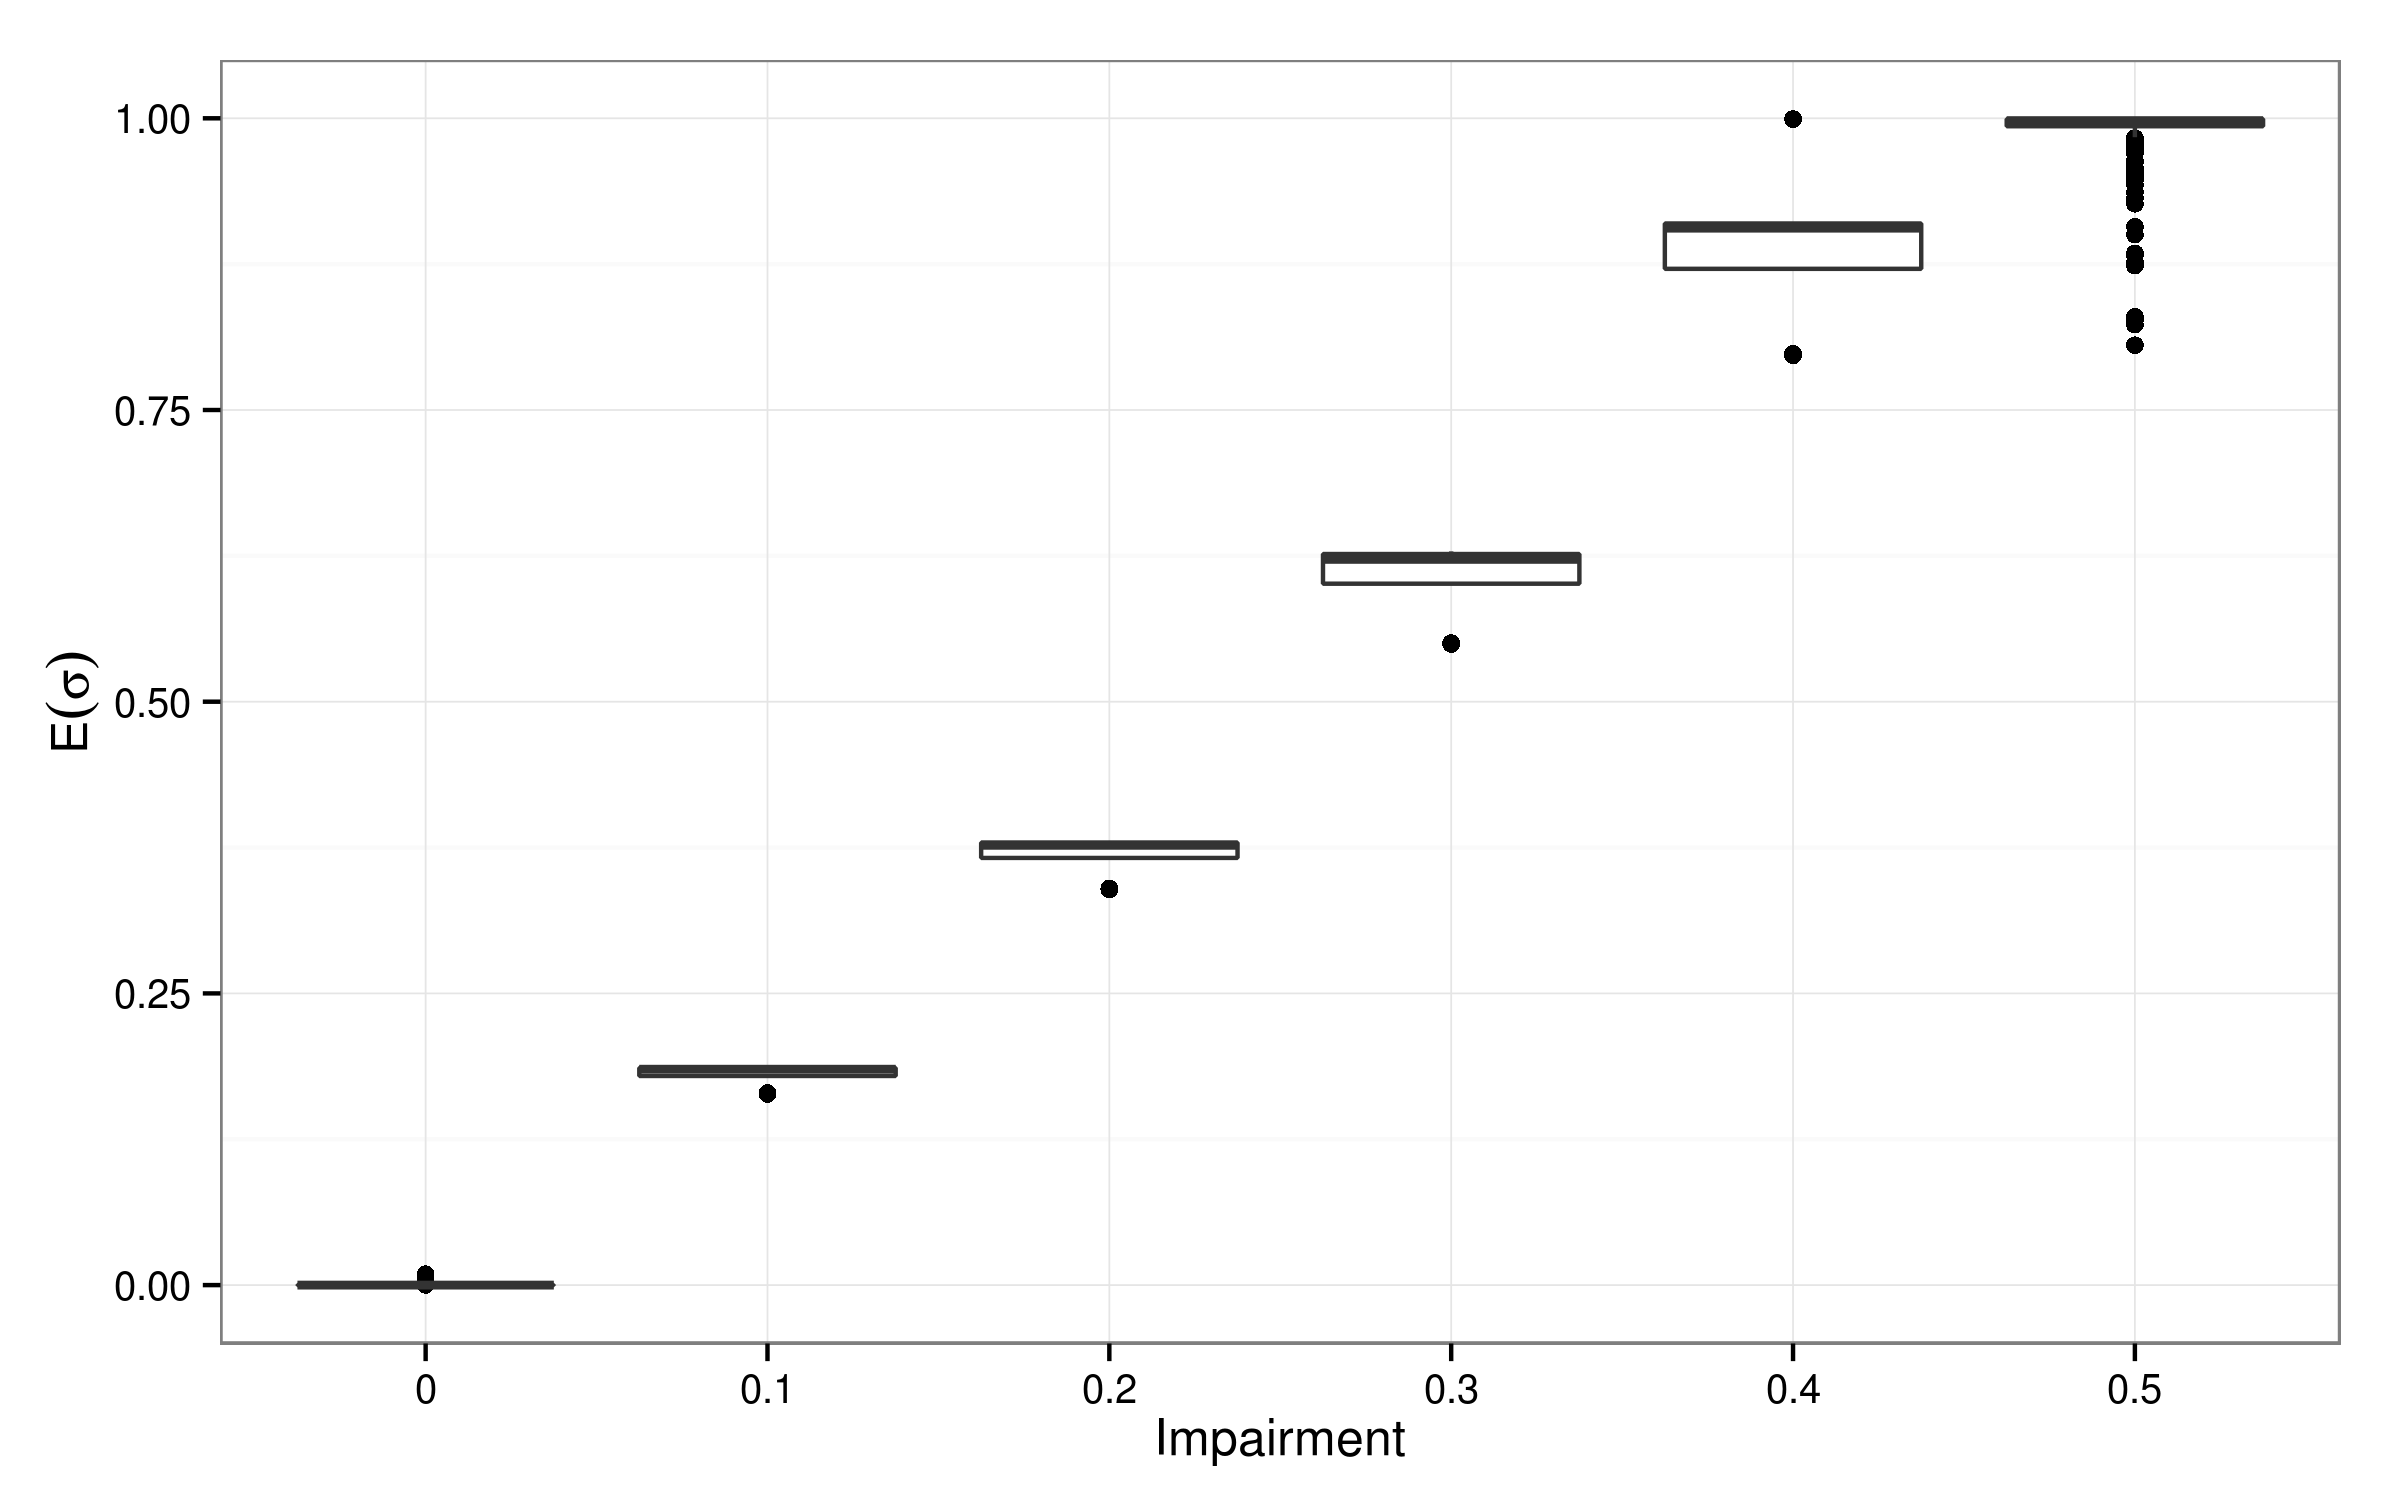
\includegraphics[width=\textwidth]{plots/Speaker-entropy-20140813-194306}
                \caption{Entropy of sender strategy.}
%                \label{fig:gull}
        \end{subfigure}
        \begin{subfigure}{0.45\textwidth}
                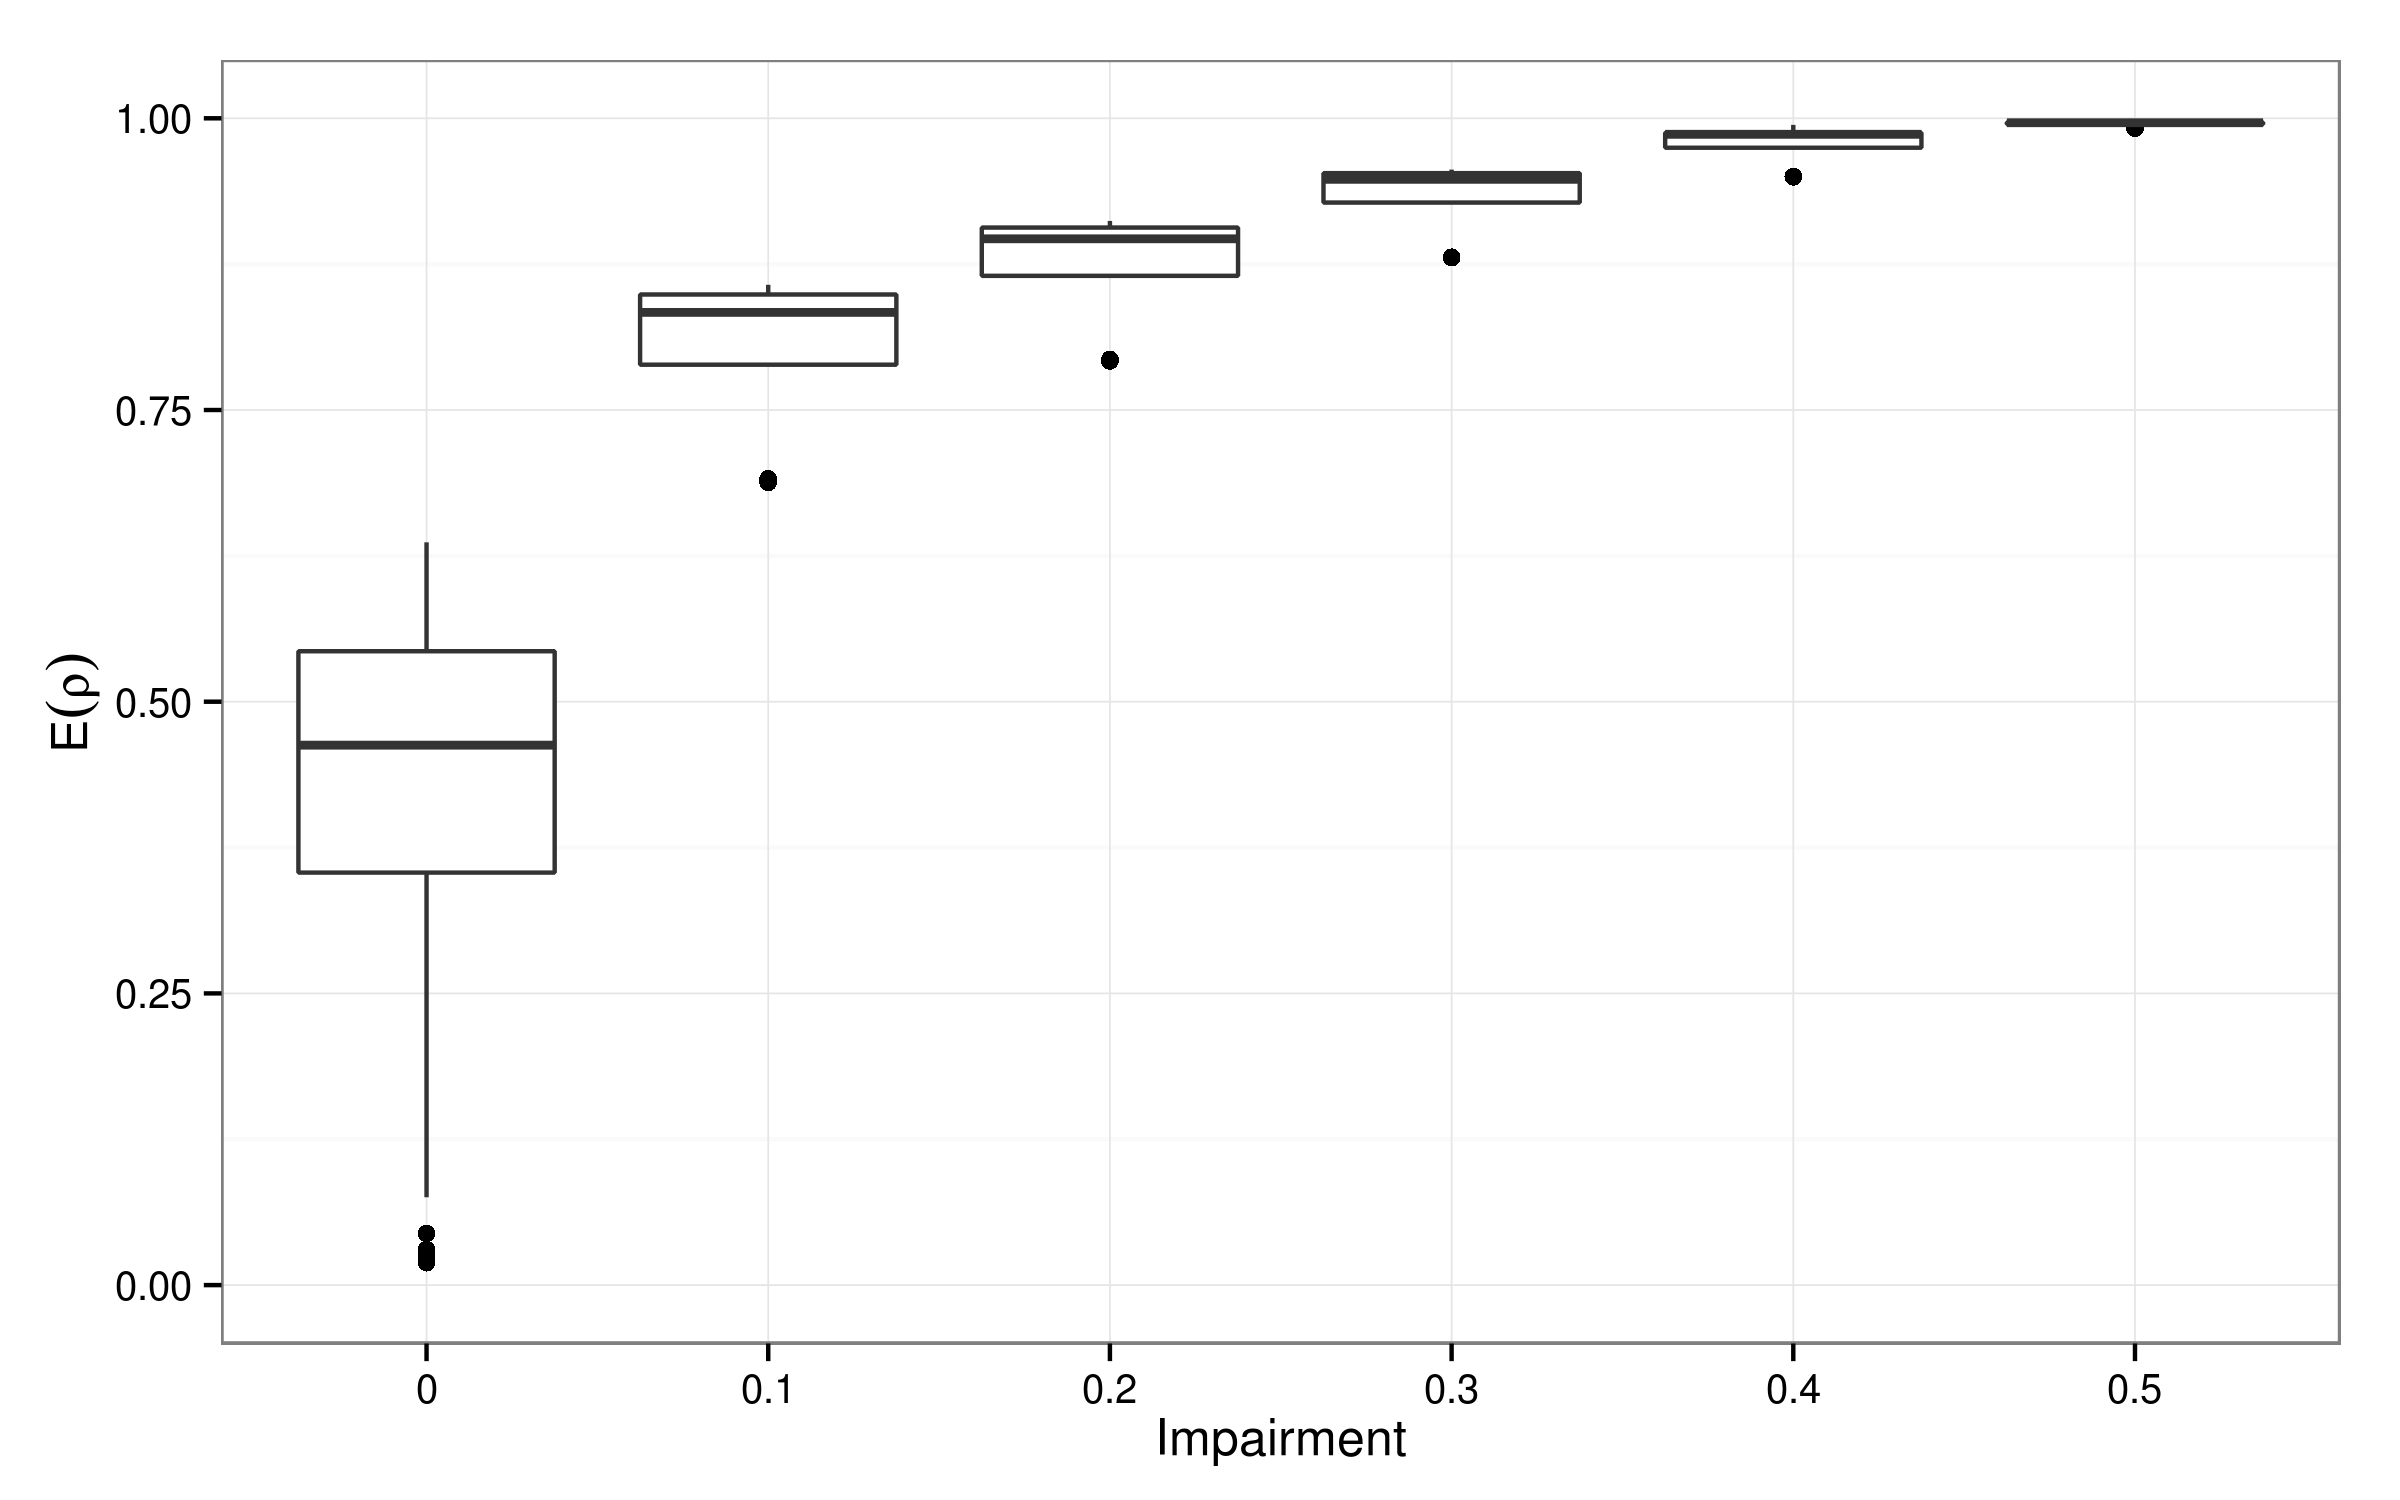
\includegraphics[width=\textwidth]{plots/Hearer-entropy-20140813-194306}
                \caption{Entropy of receiver strategy.}
        \end{subfigure}

        \begin{subfigure}{0.45\textwidth}
                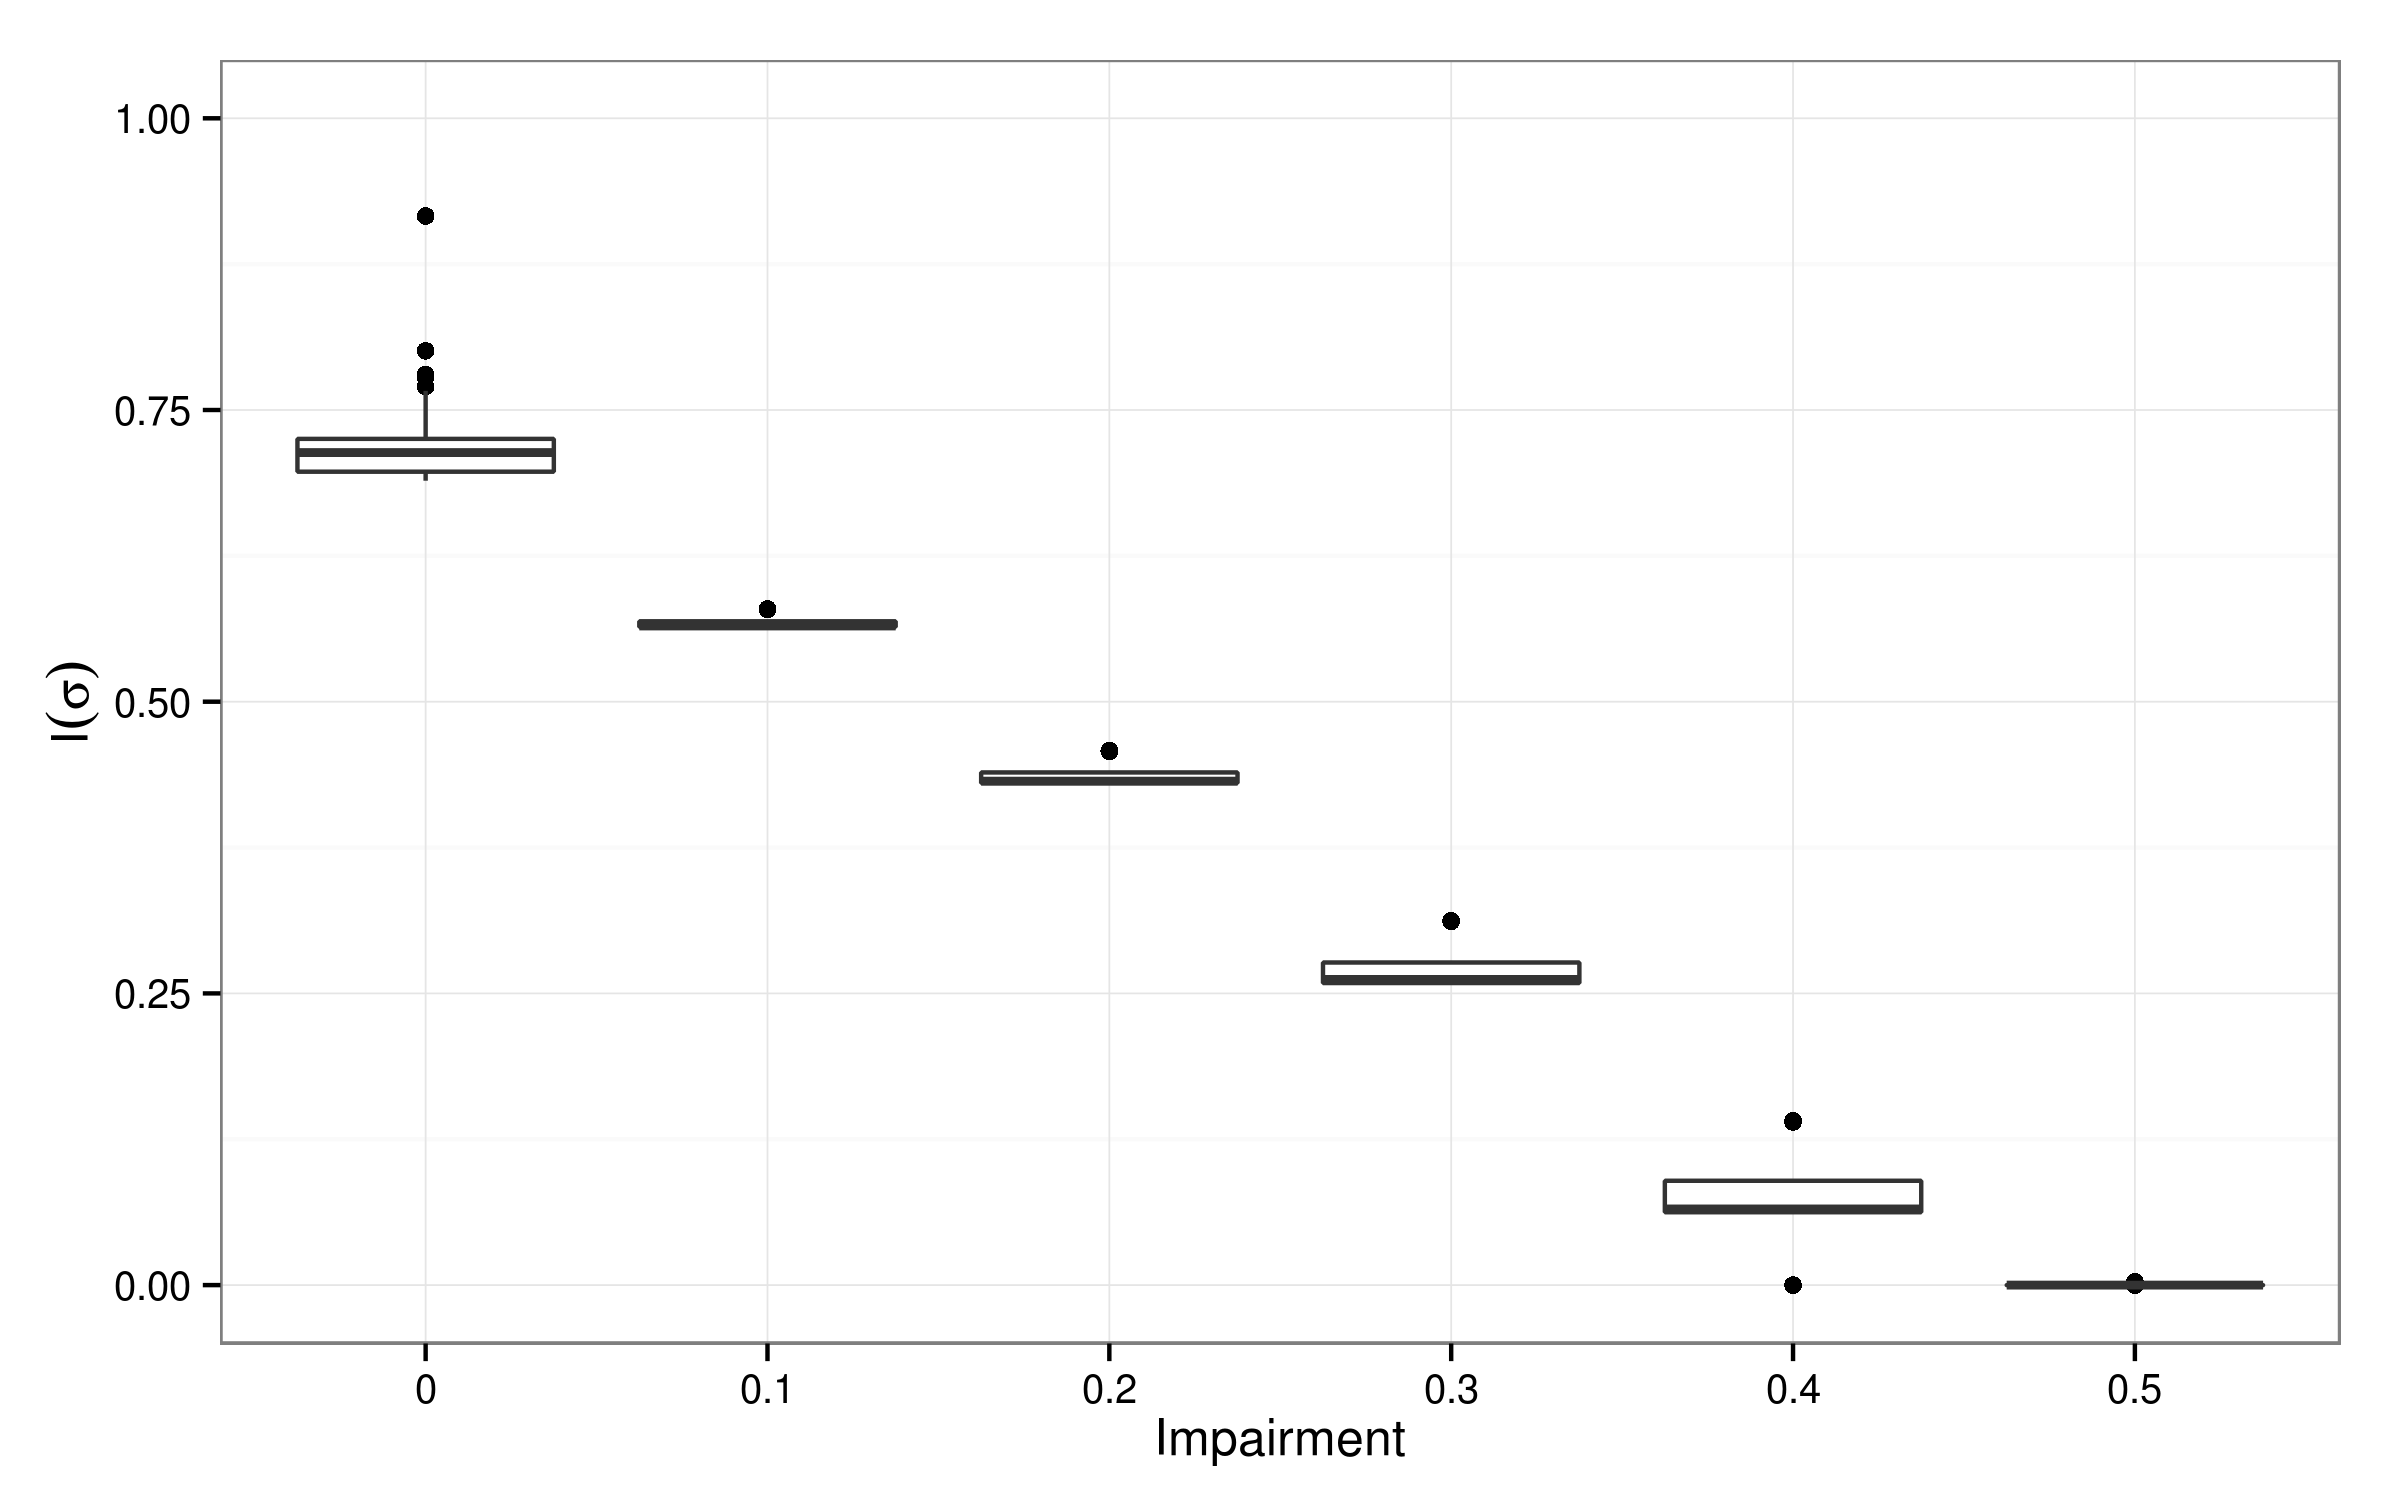
\includegraphics[width=\textwidth]{plots/Speaker-informativity-20140813-194306}
                \caption{Informativity of sender strategy.}
        \end{subfigure}
        \begin{subfigure}{0.45\textwidth}
                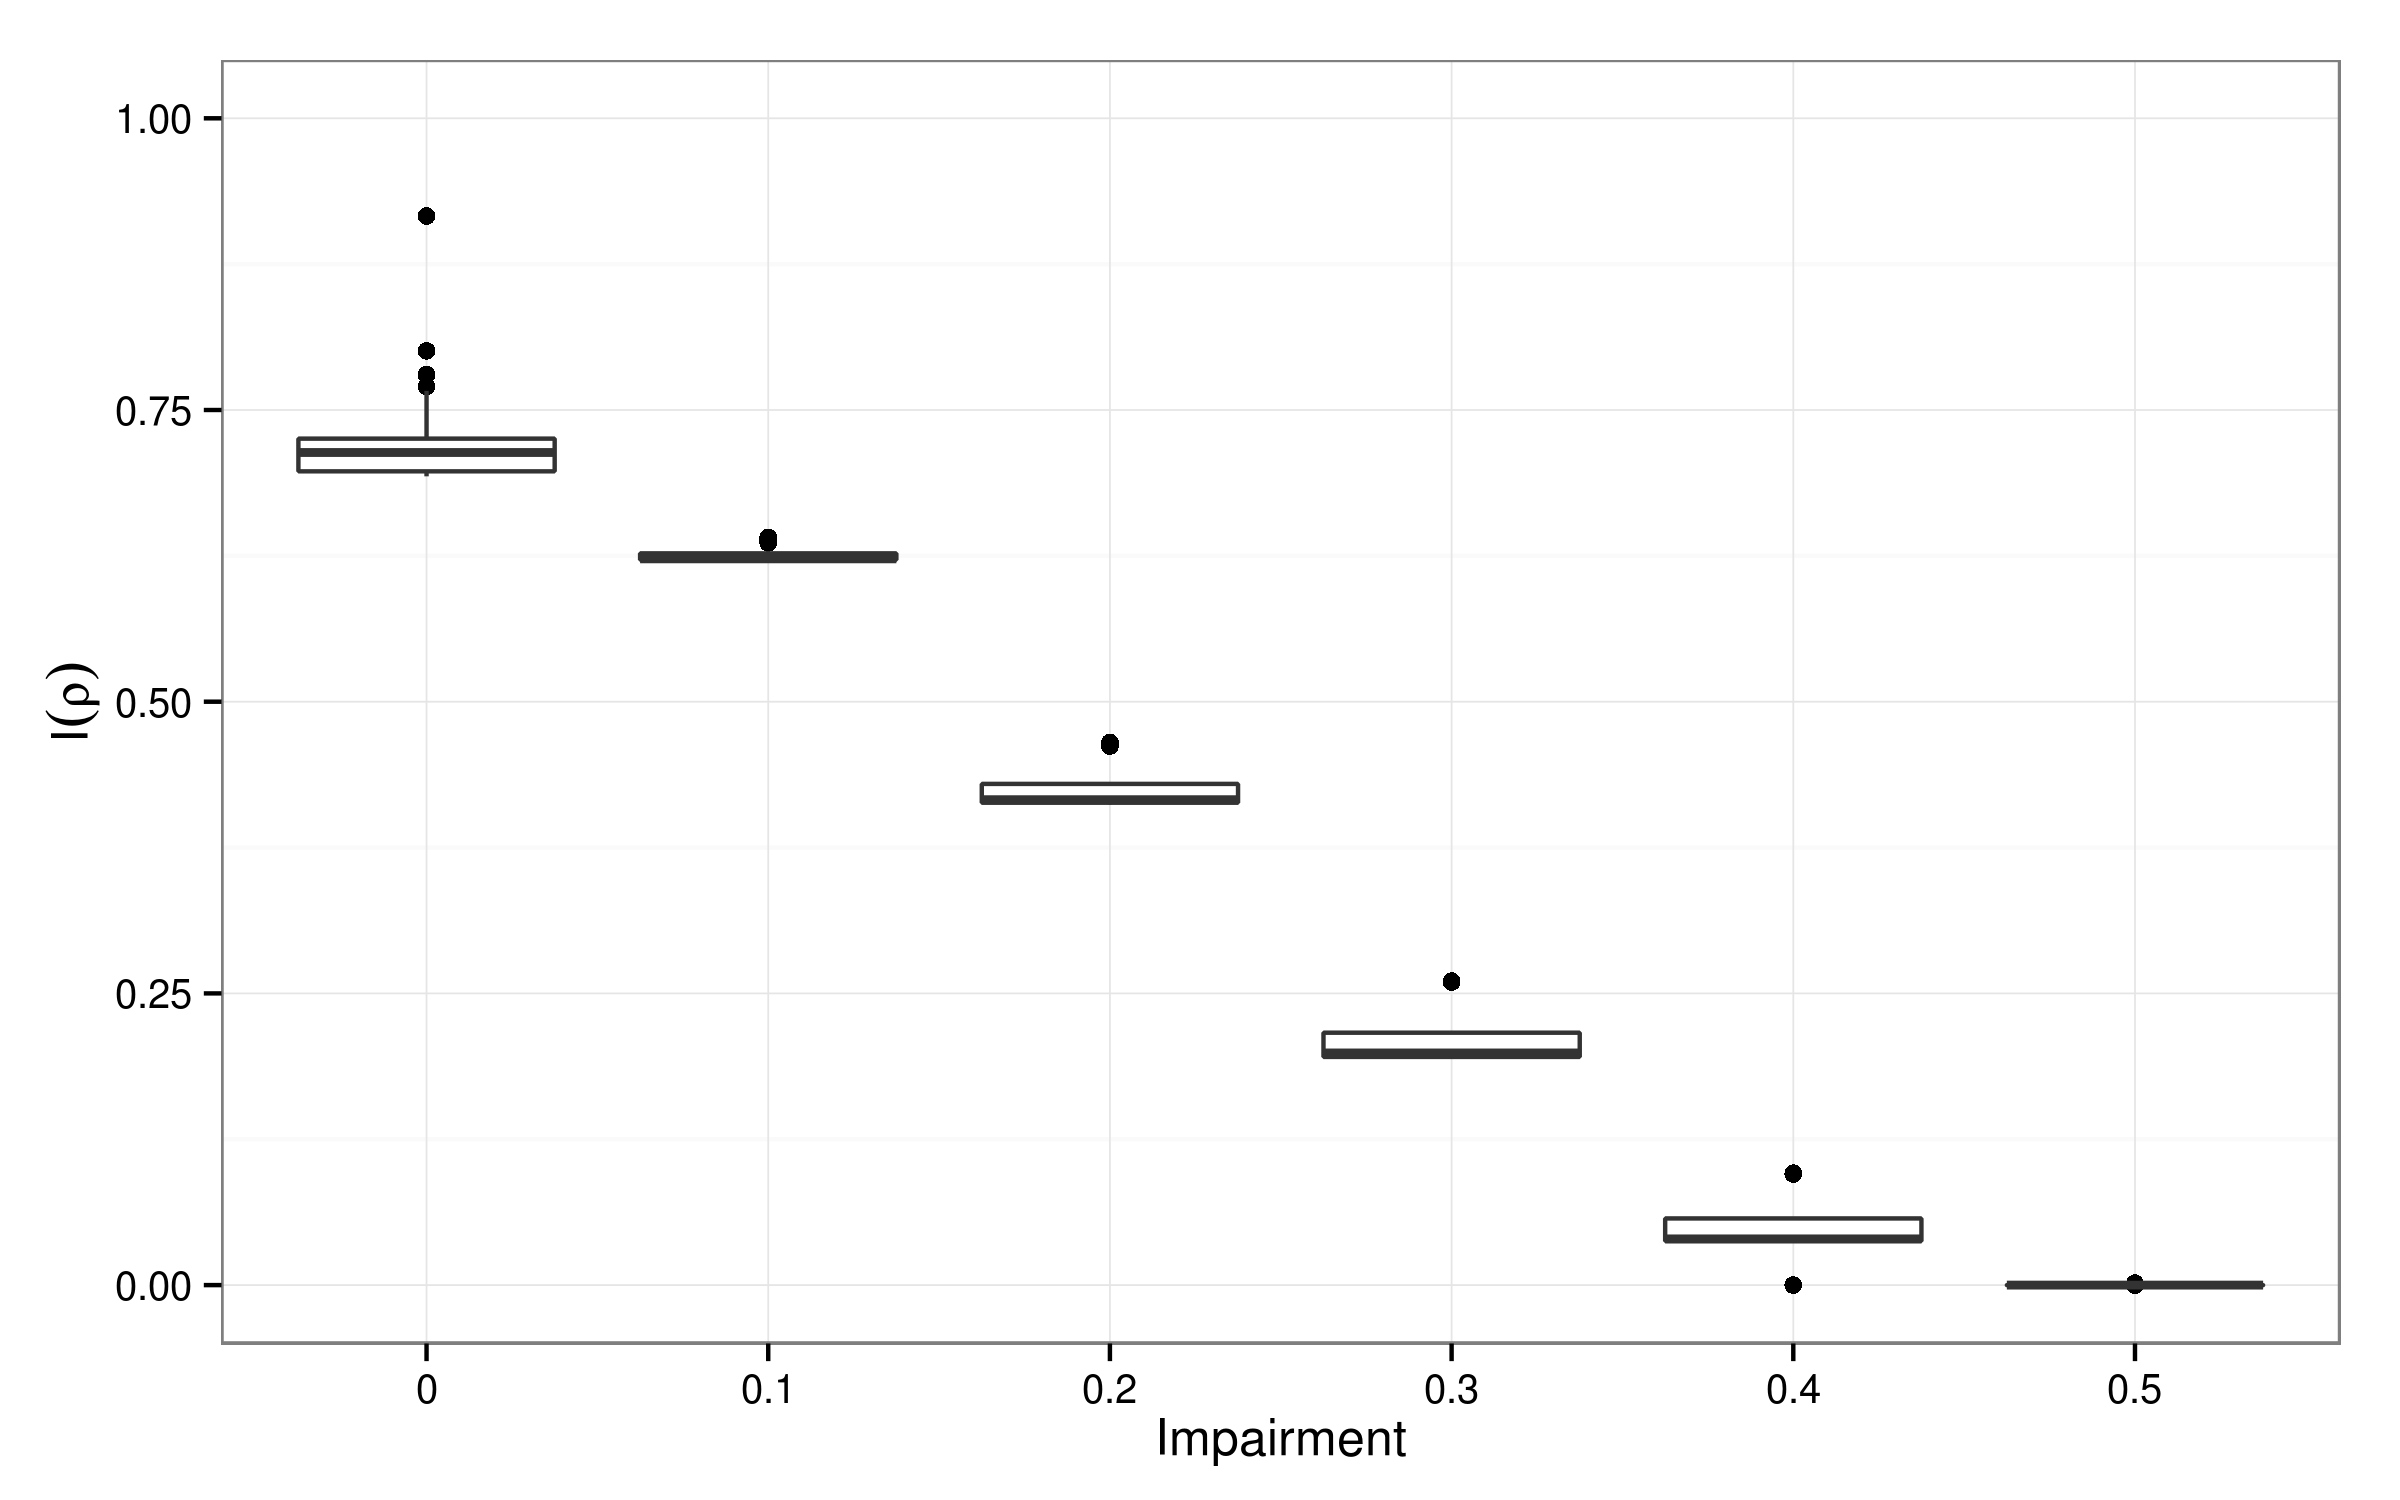
\includegraphics[width=\textwidth]{plots/Hearer-informativity-20140813-194306}
                \caption{Informativity of receiver strategy.}
        \end{subfigure}

        \begin{subfigure}{0.45\textwidth}
                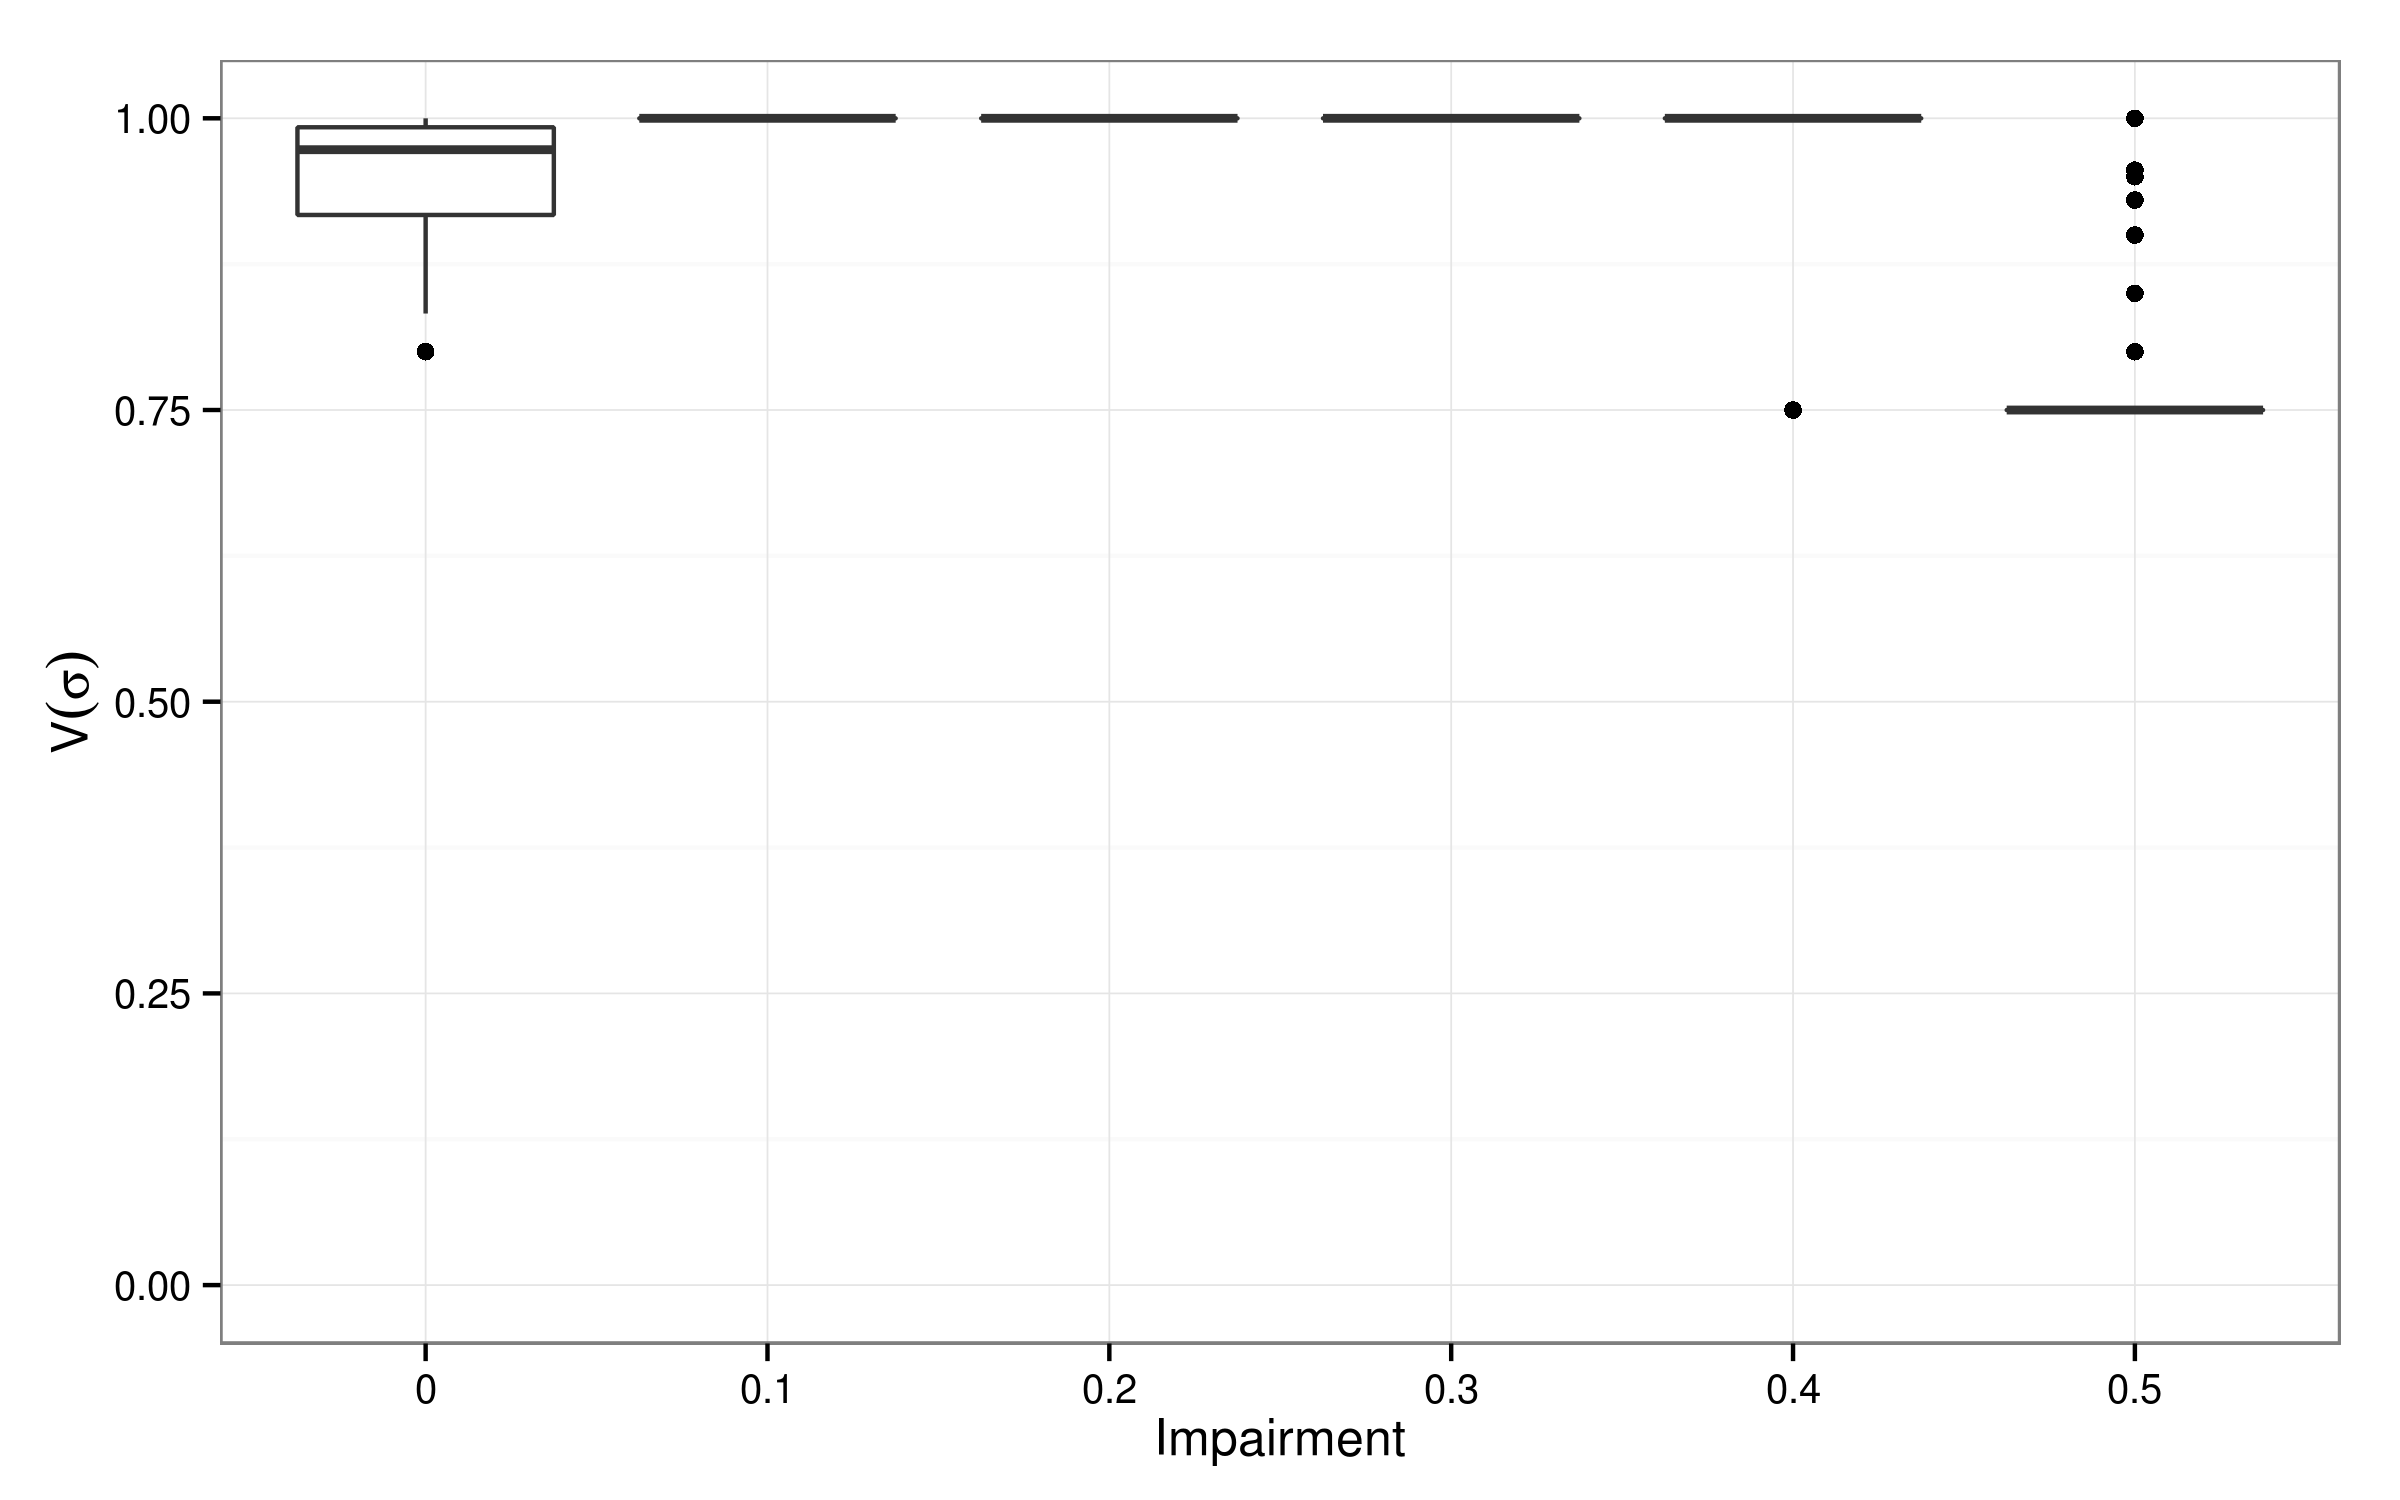
\includegraphics[width=\textwidth]{plots/Speaker-Voronoiness-20140813-194306}
                \caption{Voronoiness of sender strategy.}
        \end{subfigure}
        \begin{subfigure}{0.45\textwidth}
                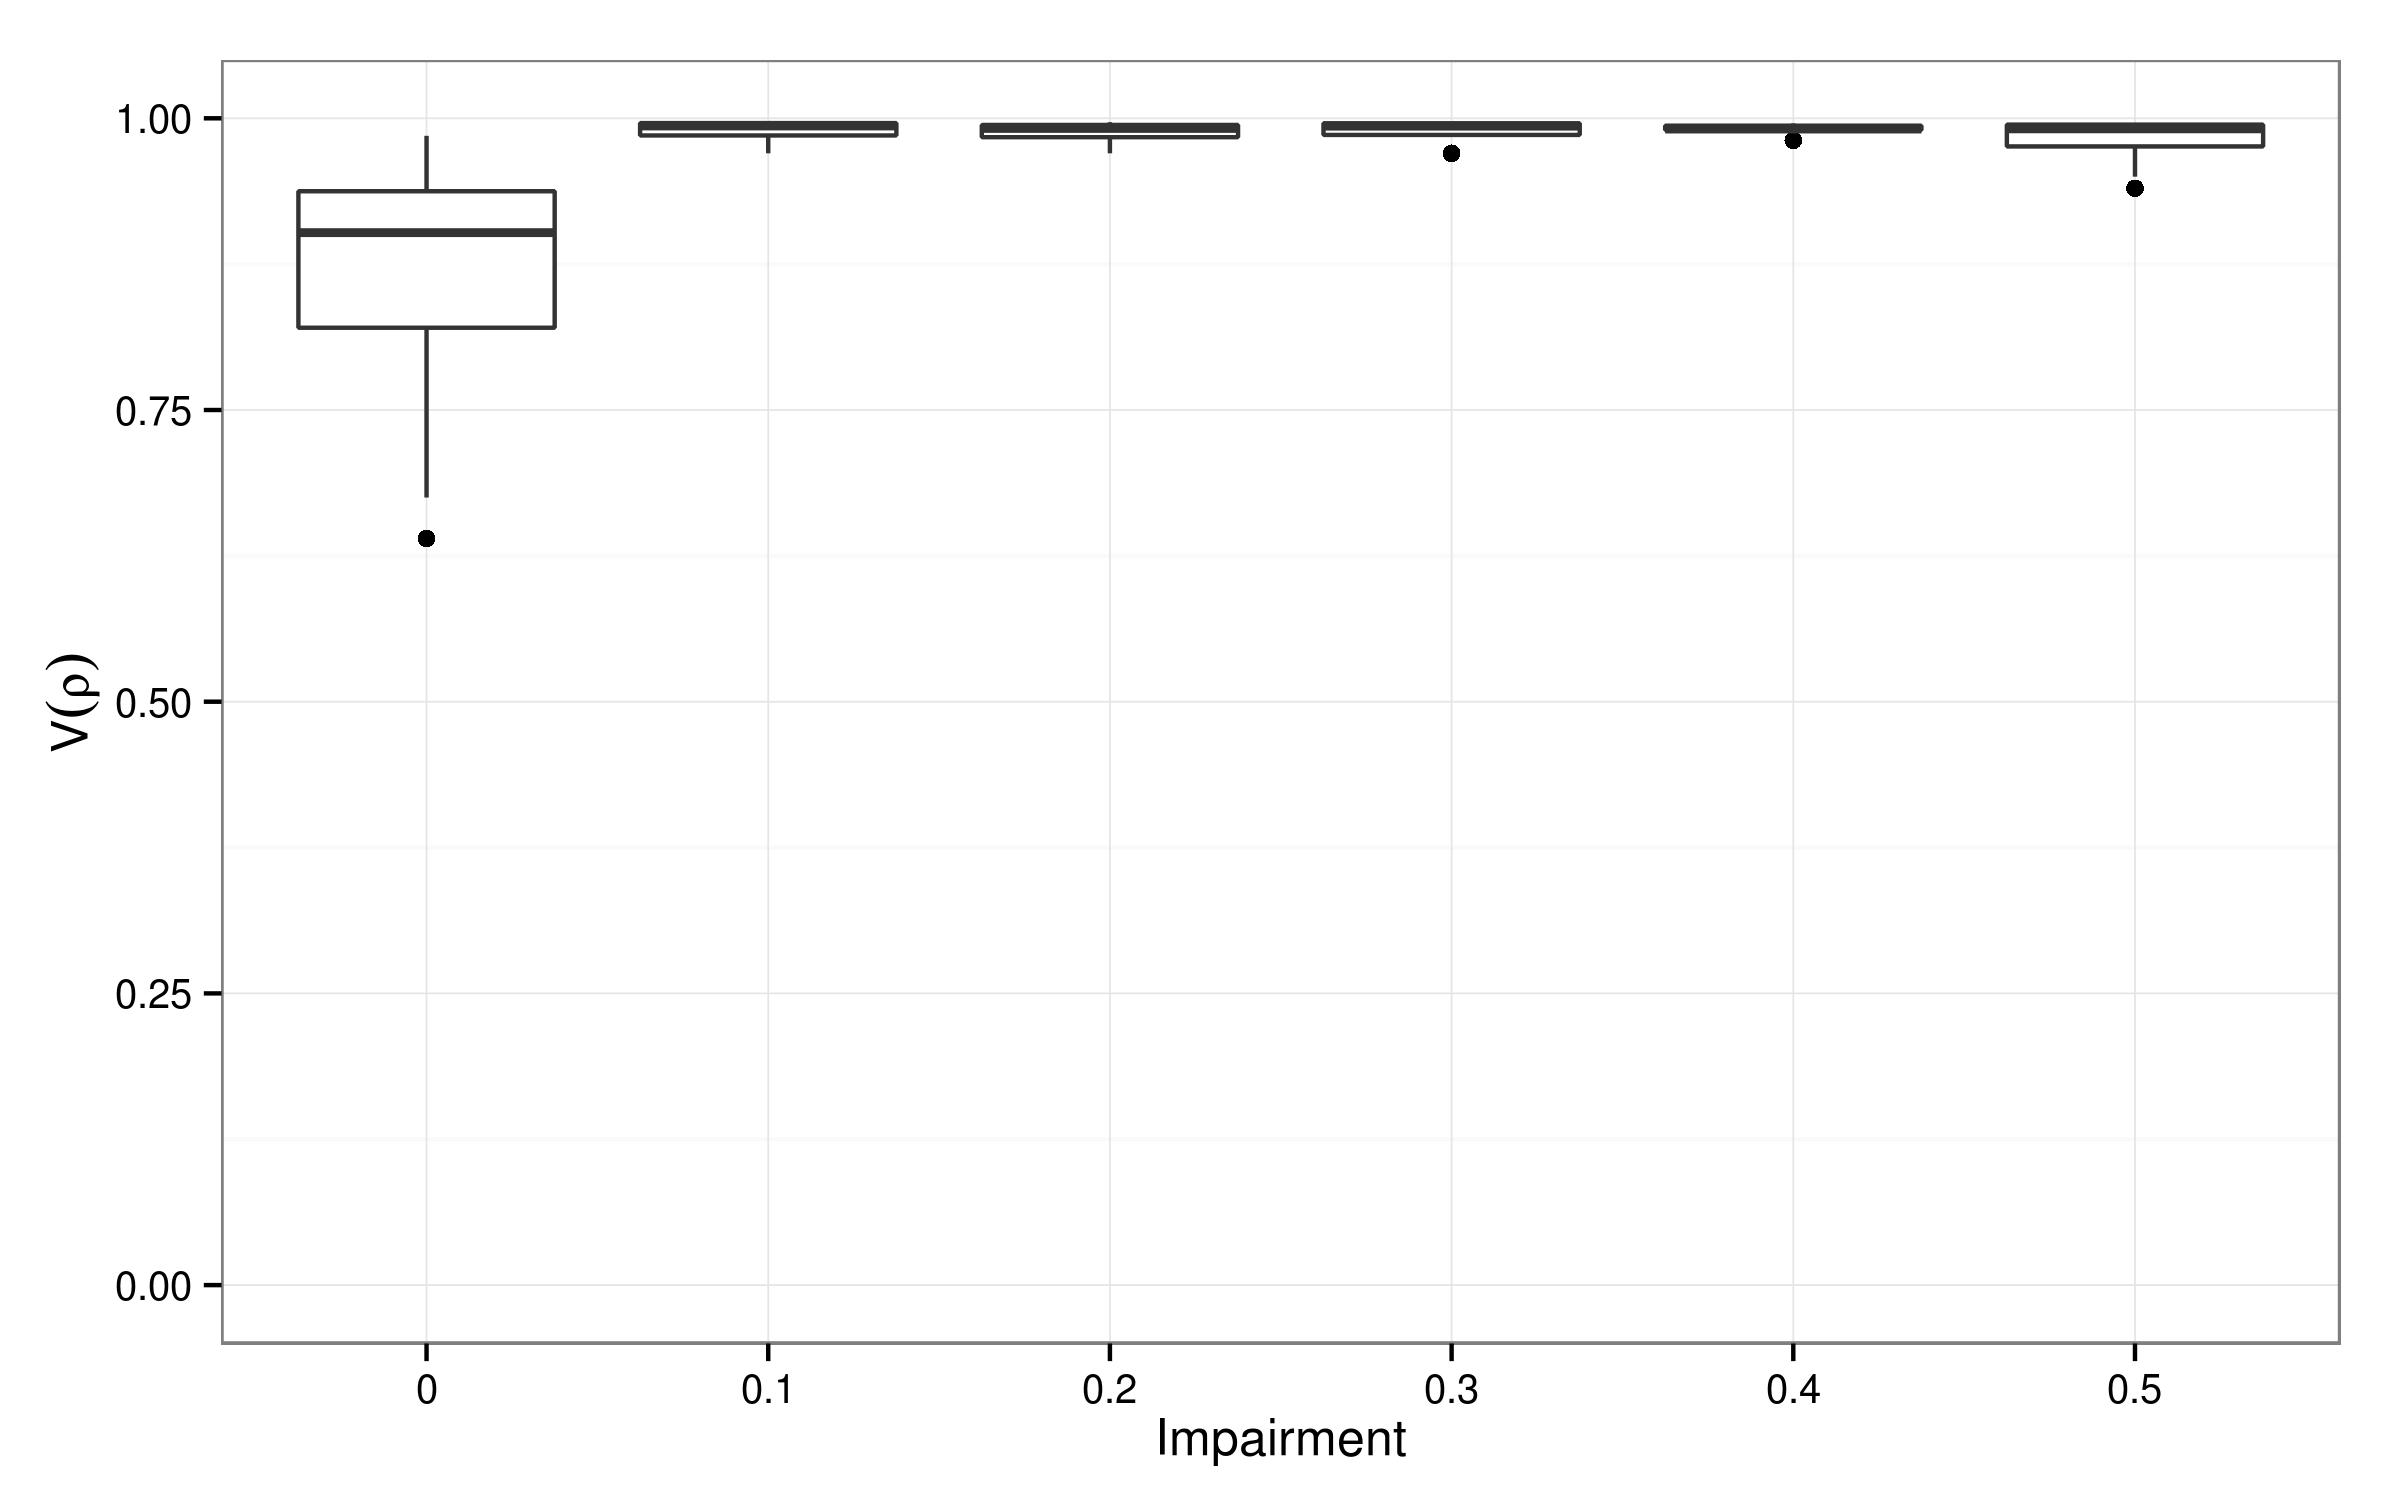
\includegraphics[width=\textwidth]{plots/Hearer-Voronoiness-20140813-194306}
                \caption{Voronoiness of receiver strategy.}
        \end{subfigure}

        \begin{subfigure}{0.45\textwidth}
                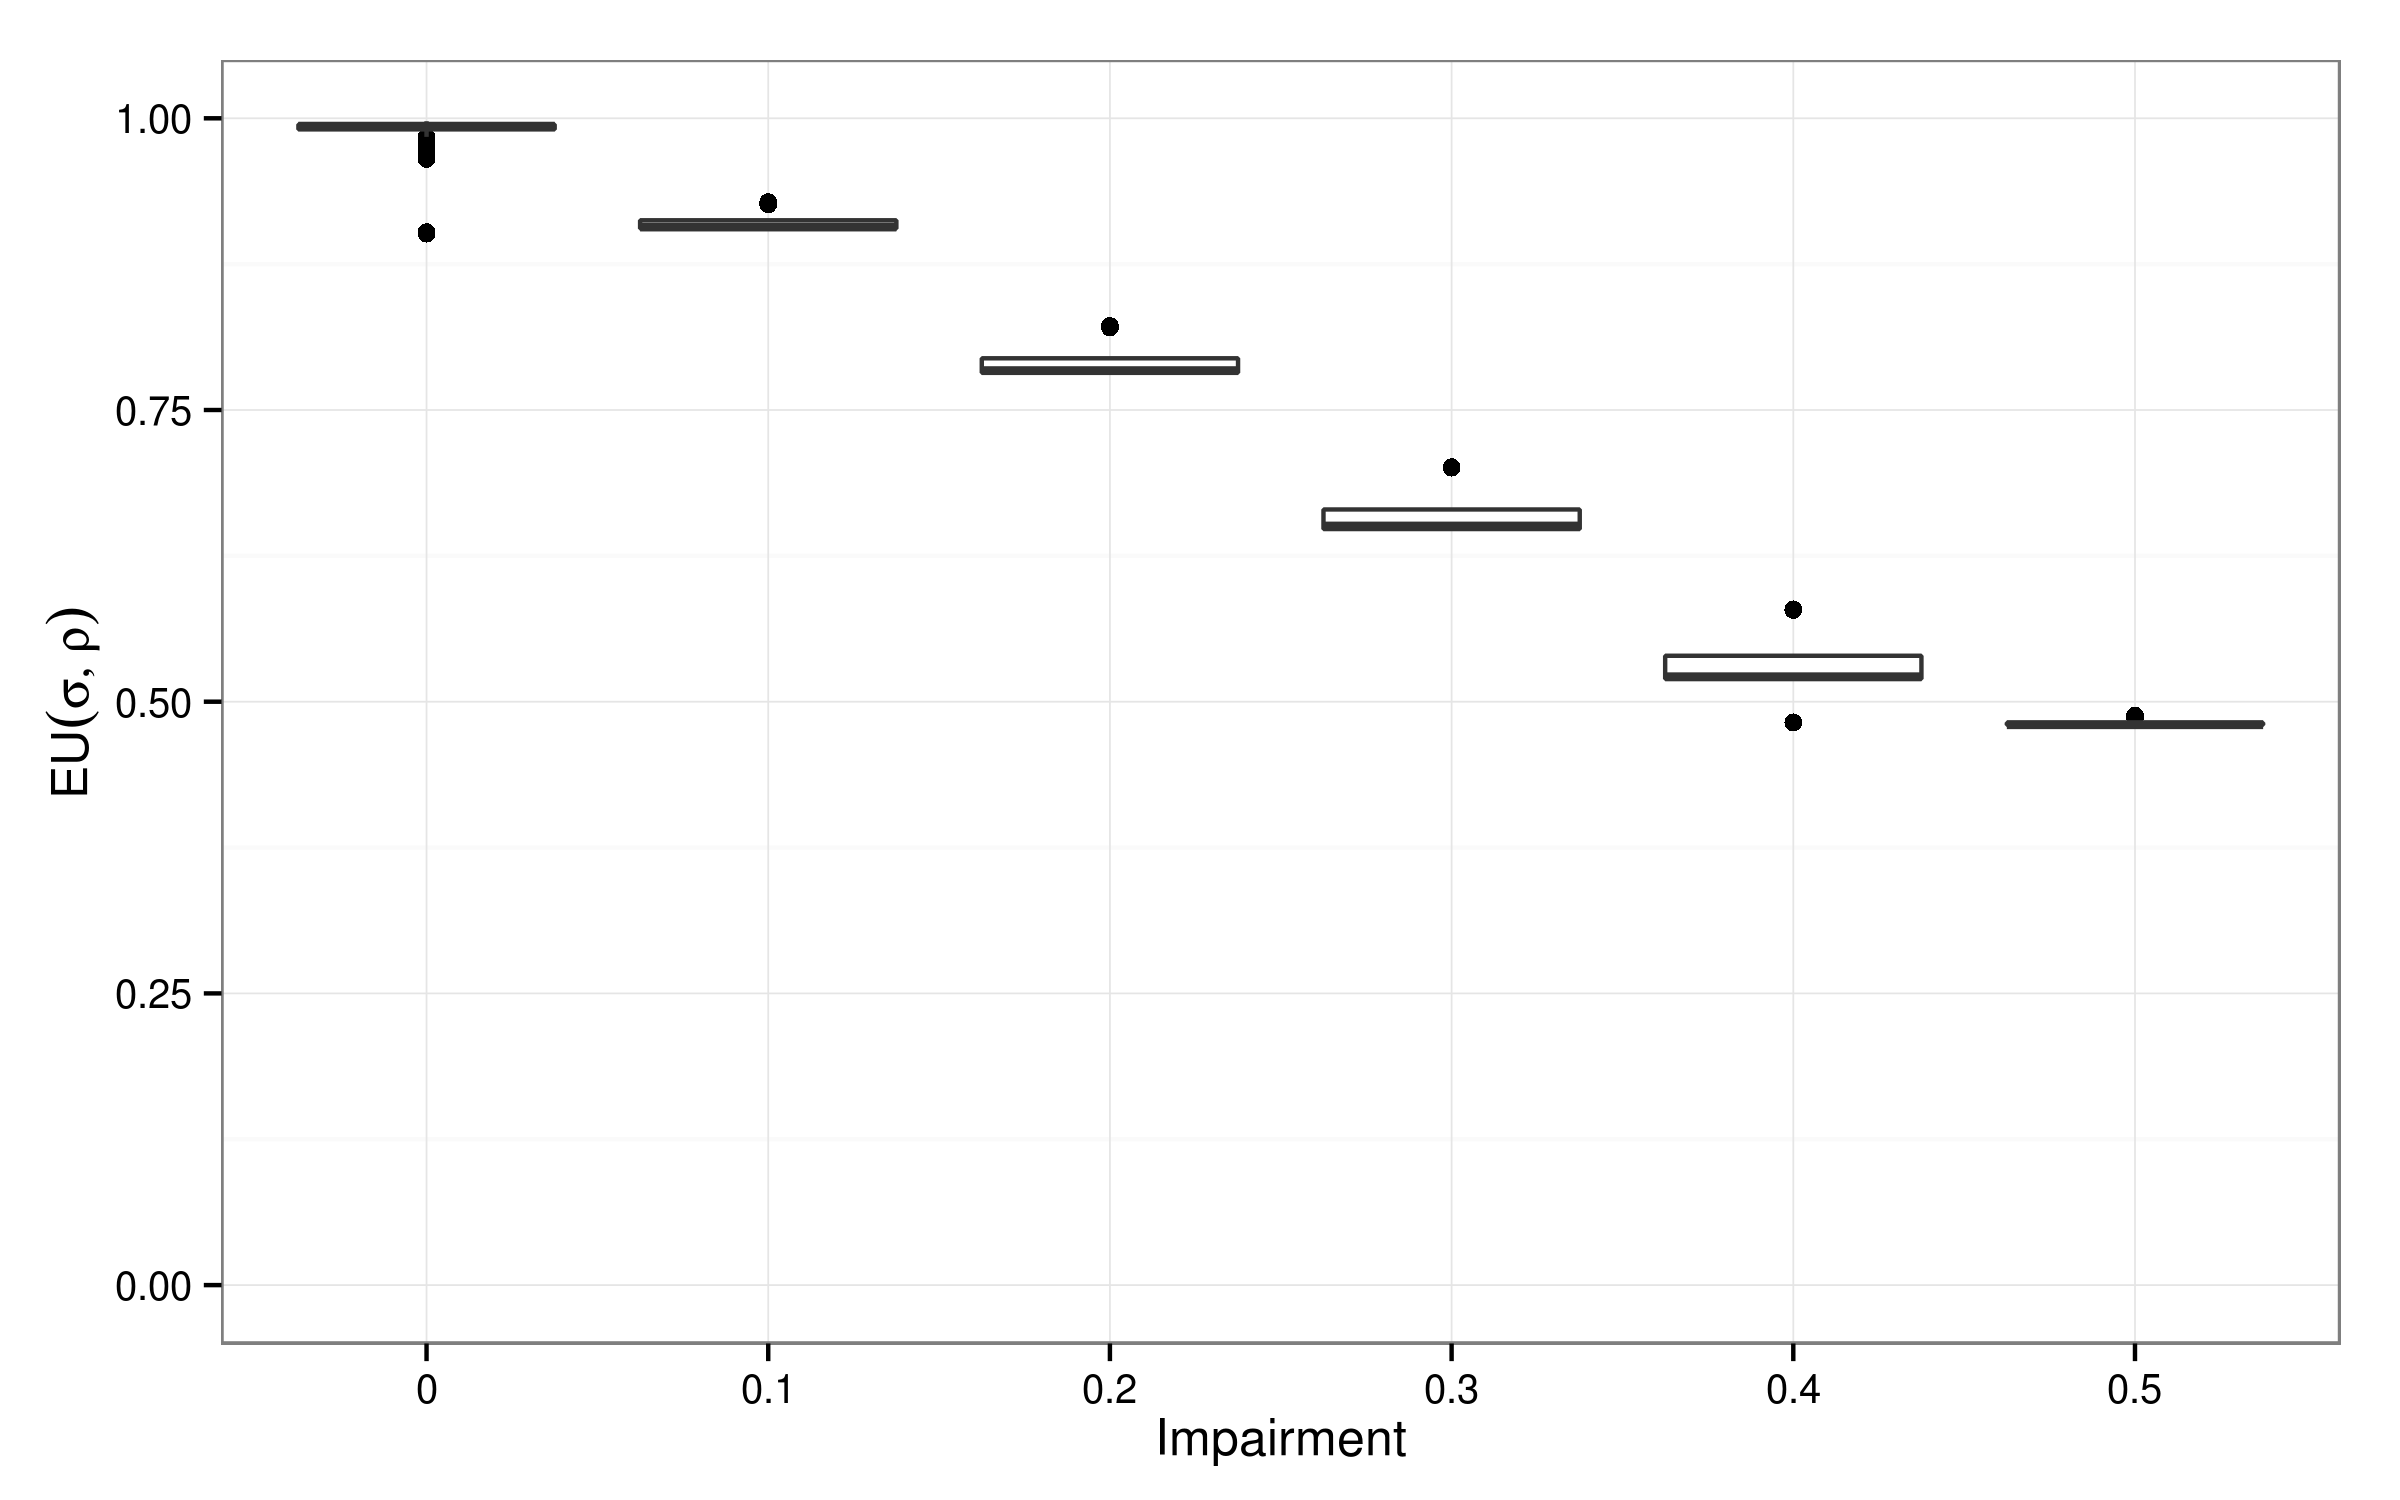
\includegraphics[width=\textwidth]{plots/Expected-utility-20140813-194306}
                \caption{Expected utility.}
        \end{subfigure}
        \begin{subfigure}{0.45\textwidth}
                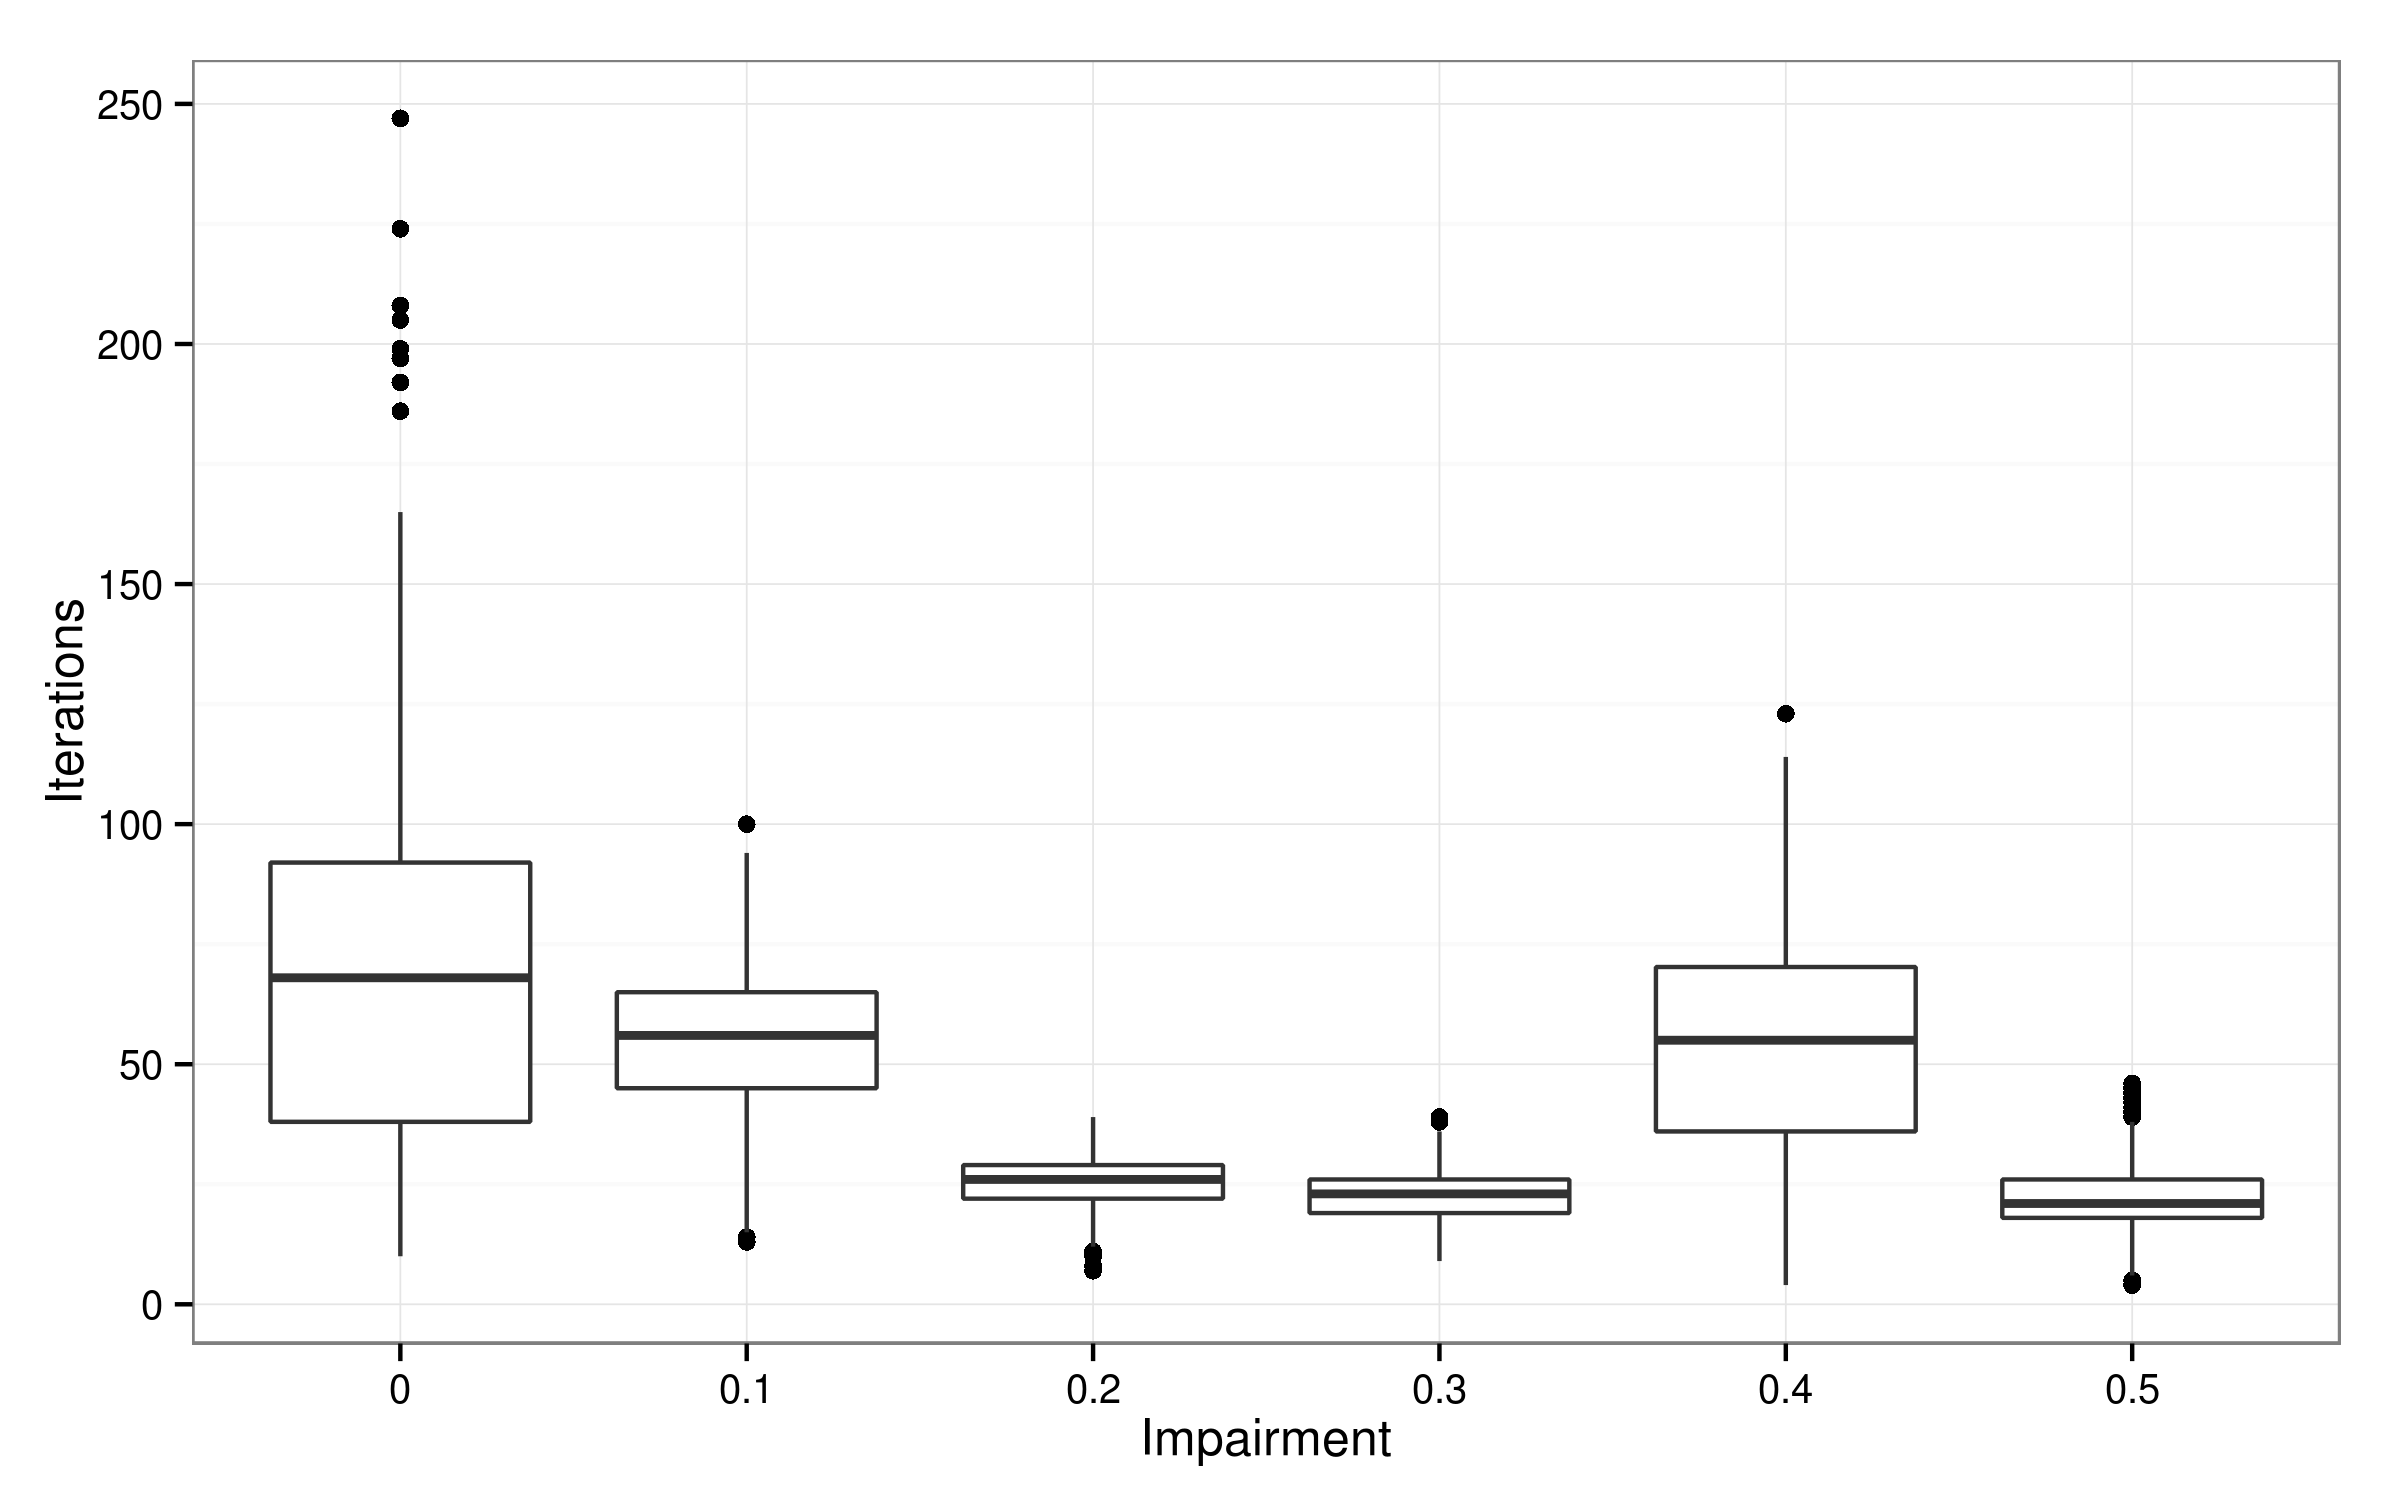
\includegraphics[width=\textwidth]{plots/Iterations-20140813-194306}
                \caption{Number of iterations until convergence.}
        \end{subfigure}
        \caption{Boxplots of metrics per impairment value.}
        \label{fig:metrics-boxplots}
\end{figure}
%
Most trends are quite clear.
Entropy seems to increase with higher impairment values for both sender and receiver.
This is an expected outcome, since the higher the impairment value, the more likely each player is to confuse two states, thus the more uncertain he will be in unequivocally associating a state with a message, or vice-versa.
The trend for informativity is also expected: more vague strategies convey less information, be it from the sender or the receiver perspective.

Regarding Voronoiness, we observe that most simulation results approximate perfect Voronoi tessalations.
This is not the case, however, for impairment of $0$ (both sender and receiver) and $0.5$ (mostly sender only).
\mytodo{JPC}{For impairment 0, the languages with the lowest sender voronoiness look like non-convex equilibria. Discuss in relation with Elliott's results?}
For impairment of $0$,  the explanation is usually that strategies can achieve a high expected utility without having perfect Voronoiness.
Although the expected long term outcome in these situations is perfect Voronoiness (given J\"ager's analytical results~\cite{Jager2007}), actually reaching it involves minor refinements which at some point do not qualify as significant change given our convergence criterion.
The result is thus an artifact of stopping the simulations before they reach perfect convergence.
For impairment of $0.5$ (and some cases with impairment of $0.4$), the reason is simply that the languages are representatives of something between babbling and pooling equilibria.
These are equilibria where $\Sstrat(\state,\messg_1) \geq \Sstrat(\state,\messg_2)$ for all $\state \in \States$, but vary from situations where $\Sstrat(\state,\messg)$ is close to $0.5$ for both messages (babbling), or is significantly higher for one of them (pooling).
\mytodo{JPC}{Plot examples}

The trend for expected utility reflects Lipman's observation that vague languages are less optimal than non-vague ones~\cite{Lipman2009:Why-is-Language}: more impairment necessarily leads to lower expected utility.
Finally, the plot for number of iterations until convergence shows that a certain level of impairment enables faster convergence.
We will discuss this further in more detail in Section~\ref{sec:discussion}.

\mytodo{JPC}{Present and discuss results per size of state space? Don't forget O'Connor's claim that speed of convergence is more important for larger \#state/\#message ratio}


%%% Local Variables: 
%%% mode: latex
%%% TeX-master: "paper"
%%% TeX-PDF-mode: t
%%% End:



